\chapter{Przeprowadzone testy}
\label{ch:tests}

$TODO$
obszerne testy, porównanie metod przy tych samych warunkach początkowych
do przeprowadzenia testów wykorzystano biblitekę jUnit, która co prawda służy do wykonywania testów jednostkowych sprawdzających poprawność pojedynczych komponentów aplikacji; bez odpalania UI, wyniki w konsoli i logach
metodyka przeprowadzenia testów
przeprowadzenie testów jest trudne i wymaga losowania środowisk i warunków i wyciągania statystyki, brak porównania do absolutu, ale można porównać różne metody w tych samych wylosowanych mapach - te same warunki początkowe
jak whca* nie zadziała, nie wiadomo, czy w ogole nie ma rozwiazania
potential field - nawet nie warto testować, raczej jako ciekawostka, nie potrafi doprowadzić do celu nawet jednego robota, screen z minimum lokalnego - studni potencjału
Na potrzeby testów do tego rozdziału Sumarycznie przeprowadzono $TODO ile$ symulacji różnych metod, w różnych warunkach, na różnych mapach.
testy powodzenia (skuteczności i wydajnosci) i testy poprawności (różnica)
histogram liczby kroków potrzebnych do rozwiązania
WHCA* z różnym parametrem okna czasowego
ustalenie maksymalnego kroku czasowego: (w + h) * 3 (robots) - arbitralnie na podstawie obserwacji liczby potrzebnych kroków
sytuacja, w której tylko jeden robot nie znalazł rozwiązania jest traktowana tak samo jako brak rozwiązania, jak gdy żaden nie znajdzie
testy ograniczać trzeba liczbą kroków symulacji, bo LRA może trwać wiecznie
po przekroczeniu liczby kroków limitu - uznanie za nieudaną
nazwa whca123
testy w bardzo trudnych środowiskach, dlatego niska skuteczność
próba 1000 i wyciąganie średniej, bo wszystko jest losowe i zależy od specyfiki układu, dlatego jedynym sensownym porównaniem jest porównywanie w tych samych warunkach

Przetestowane metody:
\begin{itemize}
	\item algorytm A* bez rozwiązywania kolizji
	\item LRA*
	\item WHCA* bez dynamicznego przydzielania priotytetów
	\item WHCA* z dynamicznym przydziałem priorytetów
	\item WHCA* z dynamicznym przydziałem priorytetów oraz dynamicznym skalowaniem okna czasowego
\end{itemize}

Zmierzone wskaźniki:
\begin{itemize}
	\item fakt doprowadzenia wszystkich robotów do celów wzdłuż bezkolizyjnych tras, skuteczność = liczba udanych / wszystkich
	\item liczba potrzebnych kroków symulacji (czas wykonywania akcji w rzeczywistym środowisku)
	\item czas wykonywania planowania (wykonywania obliczeń dla wszystkich kroków symulacji)
\end{itemize}

\section{Środowiska testowe}
Testy zostały przeprowadzone na 4 typach losowych środowisk, którym dla uproszczenia zapisu nadano nazwy:
\begin{itemize}
	\item {\bf M-15x15-5R} - mapa rozmiaru $15 \times 15$ z wygenerowanym labiryntem, 5 robotów na mapie (por. rys. \ref{fig:test-env-15-15-5}),
	\item {\bf M-15x15-10R} - mapa rozmiaru $15 \times 15$ z wygenerowanym labiryntem, 10 robotów na mapie (por. rys. \ref{fig:test-env-15-15-10}),
	\item {\bf M-35x35-5R} - mapa rozmiaru $35 \times 35$ z wygenerowanym labiryntem, 5 robotów na mapie (por. rys. \ref{fig:test-env-35-35-5}),
	\item {\bf E-15x15-40R} - mapa rozmiaru $15 \times 15$ bez przeszkód, 40 robotów na mapie (por. rys. \ref{fig:test-env-15-15-empty-40}).
\end{itemize}
Dla każdego typu środowiska za każdym razem generowana jest nowa, losowa mapa. Również położenie początkowe i docelowe robotów jest lososwane. Zatem w każdej symulacji wykorzystywane jest inne środowisko, chyba, że porównywane są między sobą różne metody. Wtedy rekonstruowane są te same warunki początkowe, aby przeprowadzić symulację ponownnie z wykorzystaniem innej metody planowania.

Każdy z robotów otrzymuje losowe położenie początkowe. Jest to zawsze pole, na którym nie znajduje się przeszkoda, ani nie ma na nim innego robota.
Punkty docelowe także są losowane. Mogą to być pola, na których obecnie znajduje się jakiś robot, natomiast nie może to być punkt docelowy należący do innego robota, gdyż w przeciwnym wypadku uniemożliwiłoby to znalezienie rozwiązania, niezależnie od metody planowania.

\begin{figure}
	\centering
	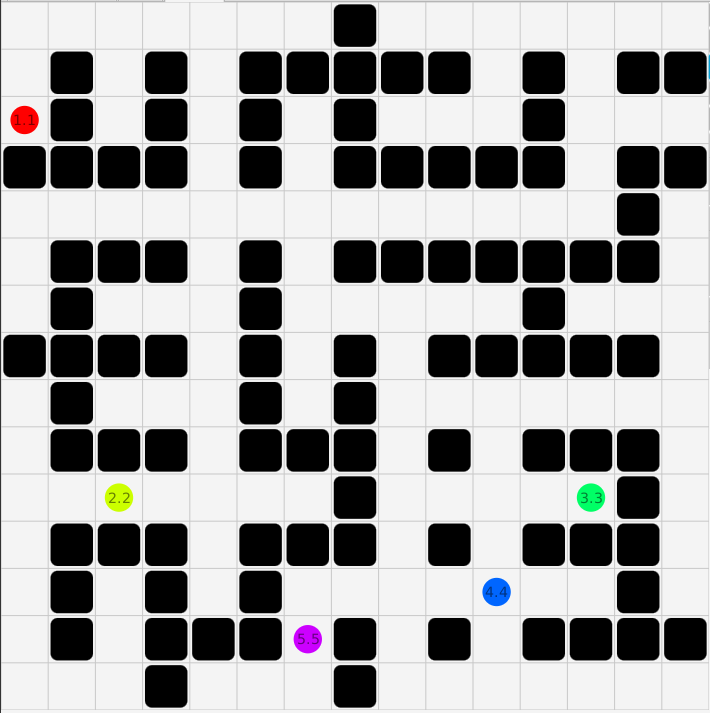
\includegraphics[width=0.6\columnwidth]{img/robopath/tests-15-15-5}
	\caption{Przykładowe środowisko typu M-15x15-5R - mapa $15 \times 15$ z wygenerowanym labiryntem, z 5 robotami w losowych położeniach}
	\label{fig:test-env-15-15-5}
\end{figure}

\begin{figure}
	\centering
	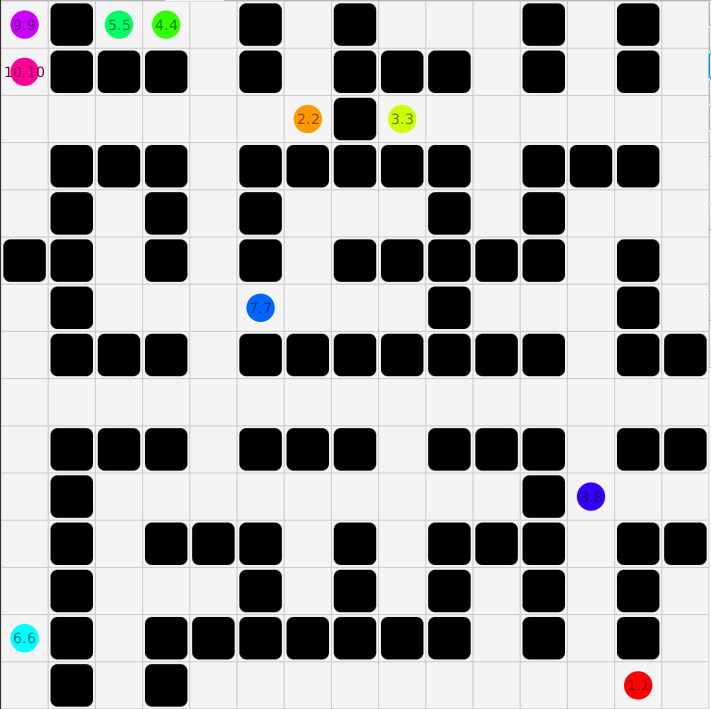
\includegraphics[width=0.6\columnwidth]{img/robopath/tests-15-15-10}
	\caption{Przykładowe środowisko typu M-15x15-10R - mapa $15 \times 15$ z wygenerowanym labiryntem, z 10 robotami w losowych położeniach}
	\label{fig:test-env-15-15-10}
\end{figure}

\begin{figure}
	\centering
	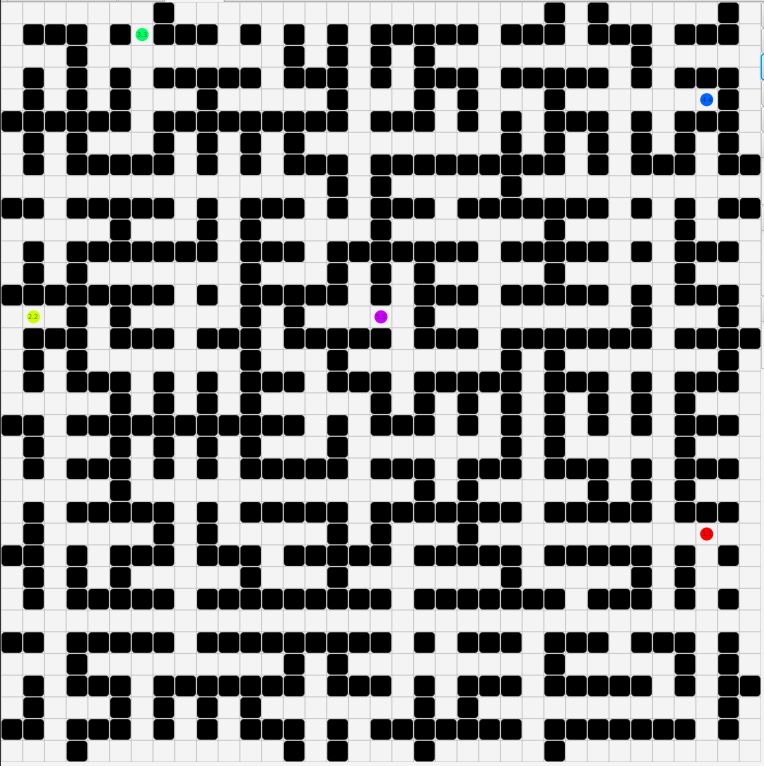
\includegraphics[width=0.6\columnwidth]{img/robopath/tests-35-35-5}
	\caption{Przykładowe środowisko typu M-35x35-5R - mapa $35 \times 35$ z wygenerowanym labiryntem, z 5 robotami w losowych położeniach}
	\label{fig:test-env-35-35-5}
\end{figure}

\begin{figure}
	\centering
	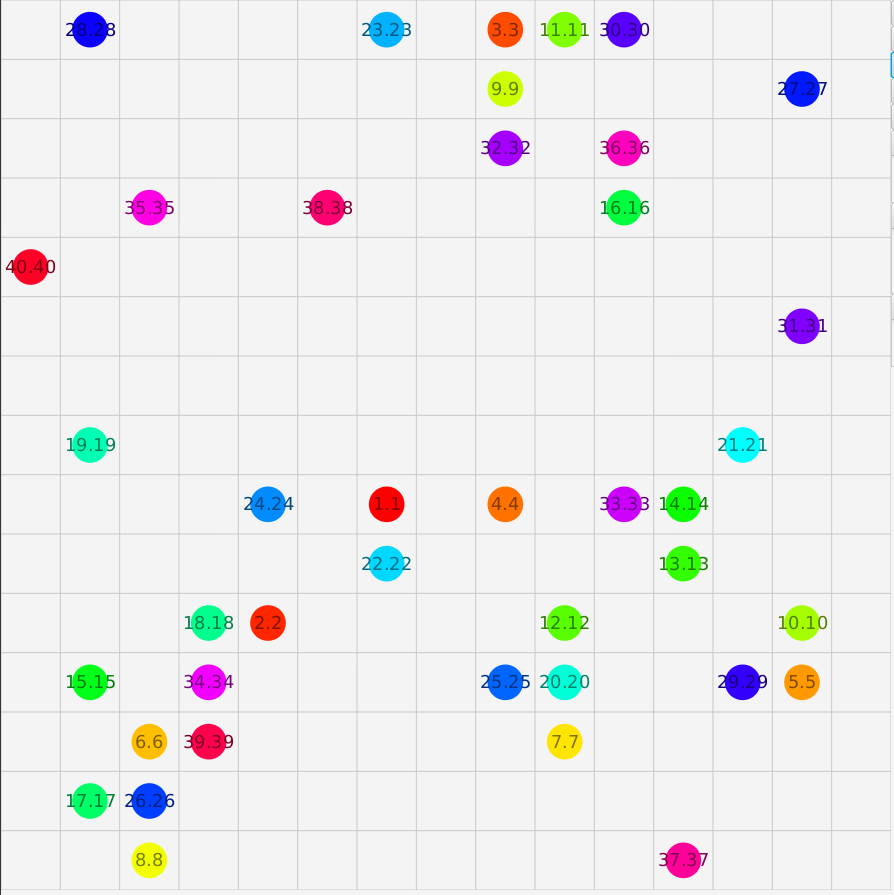
\includegraphics[width=0.6\columnwidth]{img/robopath/tests-15-15-empty-40}
	\caption{Przykładowe środowisko typu E-15x15-40R - mapa $15 \times 15$ bez przeszkód, z 40 robotami w losowych położeniach}
	\label{fig:test-env-15-15-empty-40}
\end{figure}

\section{Wyniki testów}
\subsection{Częstotliwość występowania kolizji}
Na początku przeprowadzamy testy częstotliwości występowania kolizji w badanych środowiskach.
Dla każdego robota wykonujemy planowanie trasy za pomocą prostego algorytmu A*. Następnie przeprowadzamy symulację ruchu. W momencie wykrycia kolizji robotów zatrzymujemy symulację i zliczamy ilość takich sytuacji. W ten sposób mierzymy, jak często występują kolizję miedzy robotami, jeśli planowanie odbywa się za pomocą algorytmu wyznaczania najkrótszych tras.
Możemy założyć, że algorytm A* zawsze znajdzie drogę do celu (z pominieciem pozostałych agentów), gdyż w tego typu środowiskach zawsze istnieje połaczenie miedzy dwoma dowolnymi polami na mapie.

W tabeli \ref{tab:test-collision-frequency} przedstawiono wyniki eksperymentów. Skuteczność oznacza w tym przypadku procentową liczbę symulacji, w których ruch wzdłuż zaplanowanych tras odbył się bez żadnych kolizji i wszystkie roboty zostały doprowadzone do celu.
Kolumna "Przeprowadzone symulacje" wyrażona jest w liczbie losowo wygenerowanych środowisk określonego typu.

\begin{table}
\caption{Częstotliwosć występowania kolizji w środowiskach zbadana za pomocą skuteczności algorytmu A*} \label{tab:test-collision-frequency} 
\centering
\begin{tabular}{| l | r | r | r |}
\hline
{\bf Typ środowiska} & {\bf Przeprowadzone symulacje} & {\bf Skuteczność} & {\bf Wystąpienie kolizji} \\ \hline
M-15x15-5R  & 1000 & 10\% & 90\% \\ \hline
M-15x15-10R & 1000 & 1\%  & 99\%  \\ \hline
M-35x35-5R  & 1000 & 14\% & 86\% \\ \hline
E-15x15-40R & 1000 & 0\%  & 100\%  \\ \hline
\end{tabular}
\end{table}

Uzyskane niskie wskaźniki skuteczności potwierdzają, że w tego typu mapach, problem występowania kolzji jest bardzo istotny i prosty algorytm A* nie wystarcza, aby poradzić sobie z bezkolizyjnym doprowadzeniem robotów do celów.

\subsection{WHCA* w stałych oknach czasowych}
Zbadano skuteczność metody WHCA* bez dynamicznego przydziału priorytetów w zależności od wielkości okna czasowego, które pozostaje stałe w trakcie trwania jednej symulacji.
Dla każdego badanego typu środowiska wylosowano 100 map, dla których powtórzono eksperymenty w tych samych warunkach, ale z różnymi rozmiarami okna czasowego od 1 do 30.
Dla rozmiaru okna równego 1 skuteczność metody zawsze jest zerowa, gdyż zaplanowane dla robotów ścieżki są zawsze długości 1, a pierwszym punktem ścieżki jest zawsze aktualna pozycja robota.
Uzyskane wyniki dla każdego środowiska przedstawiono na wykresach \ref{fig:test-whca-window-M-15x15-5R}, \ref{fig:test-whca-window-M-15x15-10R}, \ref{fig:test-whca-window-M-35x35-5R} i \ref{fig:test-whca-window-E-15x15-40R}.

\begin{figure}
	\centering
	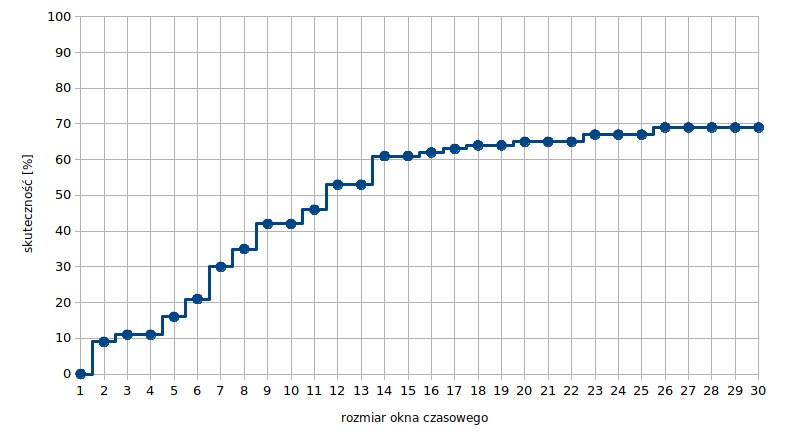
\includegraphics[width=0.8\columnwidth]{img/plots/test-whca-window-M-15x15-5R}
	\caption{Wykres skuteczności metody WHCA* w zależności od rozmiaru okna czasowego dla środowiska typu M-15x15-5R}
	\label{fig:test-whca-window-M-15x15-5R}
\end{figure}
\begin{figure}
	\centering
	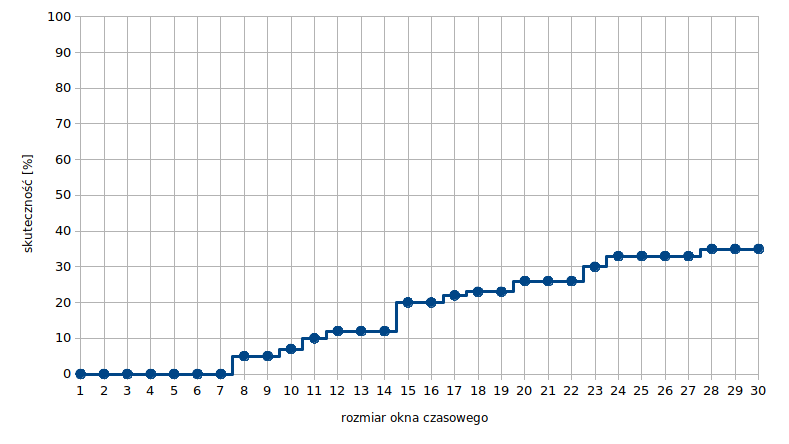
\includegraphics[width=0.8\columnwidth]{img/plots/test-whca-window-M-15x15-10R}
	\caption{Wykres skuteczności metody WHCA* w zależności od rozmiaru okna czasowego dla środowiska typu M-15x15-10R}
	\label{fig:test-whca-window-M-15x15-10R}
\end{figure}
\begin{figure}
	\centering
	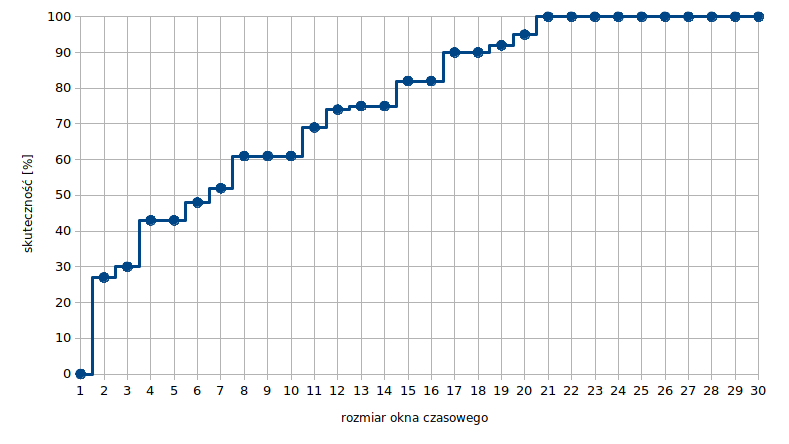
\includegraphics[width=0.8\columnwidth]{img/plots/test-whca-window-M-35x35-5R}
	\caption{Wykres skuteczności metody WHCA* w zależności od rozmiaru okna czasowego dla środowiska typu M-35x35-5R}
	\label{fig:test-whca-window-M-35x35-5R}
\end{figure}
\begin{figure}
	\centering
	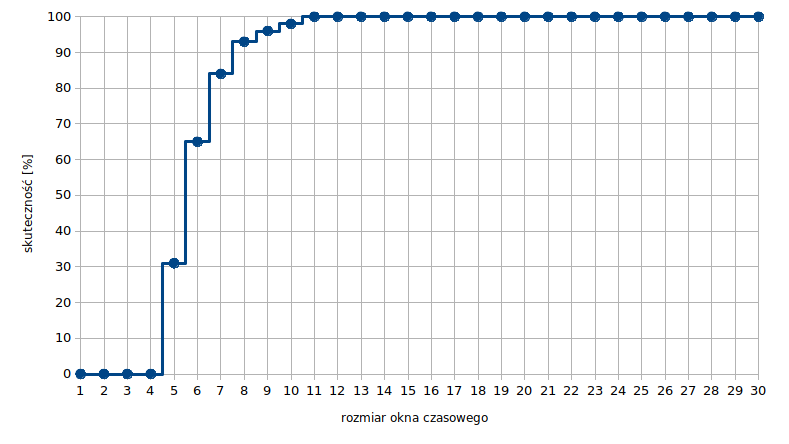
\includegraphics[width=0.8\columnwidth]{img/plots/test-whca-window-E-15x15-40R}
	\caption{Wykres skuteczności metody WHCA* w zależności od rozmiaru okna czasowego dla środowiska typu E-15x15-40R}
	\label{fig:test-whca-window-E-15x15-40R}
\end{figure}

Zgodnie z oczekiwaniami skuteczność metody WHCA* rośnie monotonicznie wraz ze wzrostem rozmiaru okna czasowego.

\subsection{Skuteczność LRA* i WHCA*}
W następnym teście przeprowadzono serie testów mających na celu porównanie skuteczności metody LRA* oraz WHCA* z dynamicznym przydziałem priorytetów.
Mapy generowane były losowo, natomiast dla każdego środowiska symulacja została wykonana dwukrotnie: raz wykonując planowanie tras metodą WHCA* a następnie metodą LRA* po odtworzeniu tych samych warunków początkowych. Dla każdej takiej symulacji zliczano, ile razy obie metody pomyślnie doprowadziły wszystkie roboty do celu, ile razy powiodła się tylko metoda WHCA*, ile razy tylko metoda LRA*, oraz ile razy żadna z metod nie powiodła się.
Umożliwiło to porównanie skuteczności metod w dokładnie tych samym warunkach. Wyniki przedstawiono w tabeli \ref{tab:test-lra-whca-effectiveness}.

\begin{table}
\caption{LRA* i WHCA* z dynamicznymi priorytetami} \label{tab:test-lra-whca-effectiveness} 
\centering
\begin{tabular}{| l | r | r | r  | r  | r |}
\hline
{\bf \shortstack{Typ\\środowiska}} &
{\bf \shortstack{Przeprowadzone\\symulacje}} &
{\bf \shortstack{Obie\\udane}} &
{\bf \shortstack{tylko WHCA*\\(dynamiczne\\priorytety)}} &
{\bf \shortstack{tylko\\LRA*}} &
{\bf \shortstack{żadna}} \\ \hline
M-15x15-5R  & 1000 & 230 (23,0\%) & 667 (66,7\%) & 0 (0\%) & 103 (10,3\%) \\ \hline
M-15x15-10R & 1000 & 12  (1,2\%)  & 640 (64,0\%) & 0 (0\%) & 348 (34,8\%) \\ \hline
M-35x35-5R  & 1000 & 513 (51,3\%) & 471 (47,1\%) & 0 (0\%) & 16  (1,6\%)  \\ \hline
E-15x15-40R & 1000 & 823 (82,3\%) & 177 (17,7\%) & 0 (0\%) & 0   (0\%)    \\ \hline
\end{tabular}
\end{table}

$TODO$ sumaryczna skuteczność

Warto zauważyć, że we wszystkich typach środowisk nie zdarzyło się, aby metoda LRA* dała lepsze rozwiazanie od WHCA*. Potwierdza to przypuszczenia, jako że metoda WHCA* jest dużo bardziej zaawansowana od metody LRA*.

\subsection{WHCA* z dynamicznym przydziałem priorytetów}
porównanie WHCA*, WHCA* + dynamiczne priorytety, WHCA* + dynamiczne priorytety + dynamiczne okno: skuteczność

poprawność malejącej skuteczności (weryfikowana podczas testów)
testowane na tych samych mapach

\begin{table}
\caption{LRA*, WHCA*, WHCA* + dynamicznymi priorytetami, WHCA* + priorytety + skalowanie okno czasowe} \label{tab:test-lra-whca-whca2-effectiveness} 
\centering
\begin{tabular}{| l | r | r | r  | r  | r |}
\hline
{\bf \shortstack{Typ\\środowiska}} &
{\bf \shortstack{Przeprowadzone\\symulacje}} &
{\bf \shortstack{Skuteczność\\WHCA*3}} &
{\bf \shortstack{Skuteczność\\WHCA*2}} &
{\bf \shortstack{Skuteczność\\WHCA*1}} &
{\bf \shortstack{Skuteczność\\LRA*}} \\ \hline
M-15x15-5R  & 1000 & 435/500 & 273/500 & 132/500 & 113/500  \\ \hline
M-15x15-10R & 1000 & 272/500 & 244/500 & 17/500  & 1/500    \\ \hline
M-35x35-5R  & 1000 & 493/500 & 349/500 & 200/500 & 264/500  \\ \hline
E-15x15-40R & 1000 & 150/150 & 150/150 & 150/150 & 115/150  \\ \hline
\end{tabular}
\end{table}
$TODO$ zmienić na /1000  i na procenty

czasem lra by lepszy od whca1 i whca2

\subsection{porównanie 2}
1) dla wszystkich, wykres skuteczności 4 algorytmów (serie):
	z labirytntem:
		- w funkcji liczby robotów (15x15) (1-30) * 100 symulacji (3000 sym)
			effect-maze-robots
		- w funkcji rozmiaru mapy (5 robotów) (3x3 - 40x40) * 100 symulacji
			effect-maze-size
	pusta mapa:
		- w funkcji liczby robotów (6x6) (1-30) * 100 symulacji (3000 sym)
			effect-empty-robots
		- w funkcji rozmiaru mapy (5 robotów) (3x3 - 40x40) * 100 symulacji
			effect-empty-size

zachowanie nierówności: WHCA*1 <= WHCA*2 <= WHCA*3
przy wyższych wartościach robotów się zlewają, bo początkowe okno czasowe jest większe
na pustej mapie WHCA*23 dają radę, ale ilość kroków jest duża
zamieszczać też tabelki?

2) dla wszystkich, wykres 4 algorytmów (serie):
	z labirytntem:
		- w funkcji liczby robotów (15x15) (1-30) * 100 symulacji (3000 sym)
			- średnia liczba kroków (dla udanych)
			- średni czas planowania (dla udanych)
			- skuteczność
				steps-maze-robots
		- w funkcji rozmiaru mapy (5 robotów) (3x3 - 40x40) * 100 symulacji
			- średnia liczba kroków (dla udanych)
			- średni czas planowania (dla udanych)
			- skuteczność
				steps-maze-mapsize

-- są to tylko przypadki w których udało się LRA, czyli proste układy
pomiar czasu może być obarczony błędami wynikającymi z narzutu JVM i działania Garbage Collectora


\subsection{Metoda pól potencjałowych}
$TODO$

\section{Charakterystyczne przypadki}
$TODO$ screeny ciekawych przypadków

\begin{figure}
	\centering
	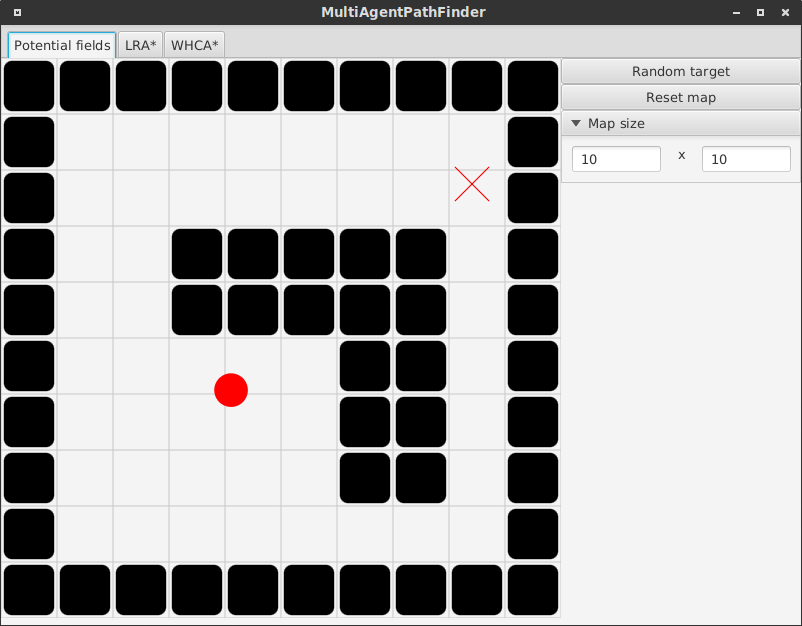
\includegraphics[width=0.8\columnwidth]{img/robopath/field-potential-hole}
	\caption{Robot uwięziony w studni potencjału. Zerowa siła wypadkowa nie pozwala mu dotrzeć do celu.}
	\label{fig:test-field-potential-hole}
\end{figure}

\begin{figure}
	\centering
	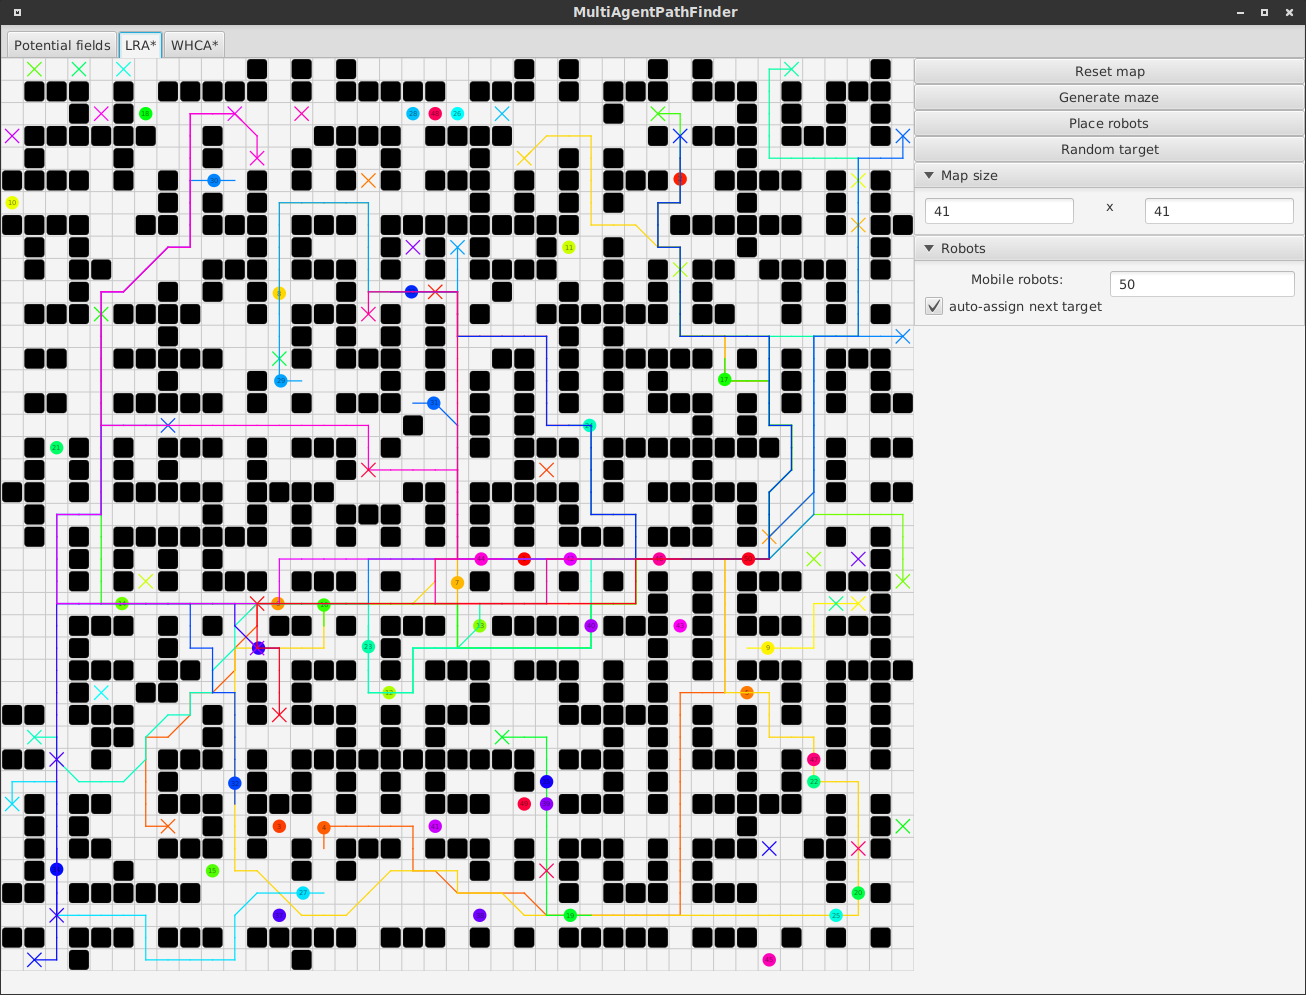
\includegraphics[width=0.8\columnwidth]{img/robopath/lra-bigmap}
	\caption{Metoda LRA*: duża mapa z dużą liczbą robotów}
	\label{fig:test-lra-bigmap}
\end{figure}

% \begin{figure}
% 	\centering
% 	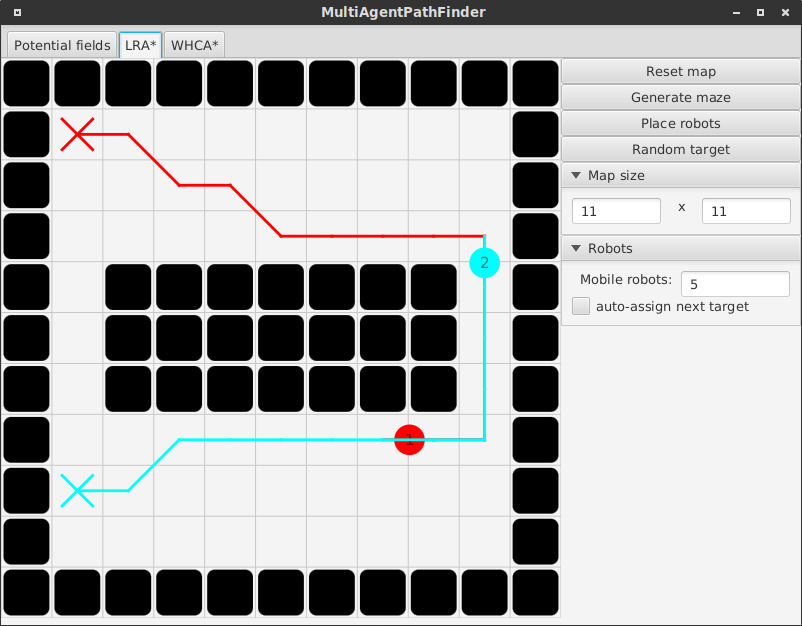
\includegraphics[width=0.8\columnwidth]{img/robopath/lra-cycle}
% 	\caption{Metoda LRA*: 2 roboty w cyklu akcji}
% 	\label{fig:test-lra-cycle}
% \end{figure}

\begin{figure}
	\centering
	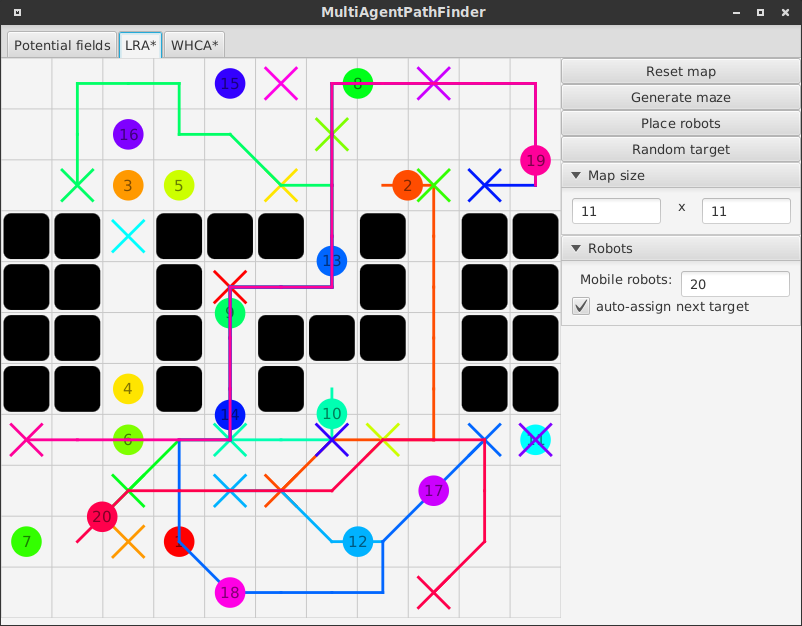
\includegraphics[width=0.8\columnwidth]{img/robopath/lra-lot-robots}
	\caption{Metoda LRA*: dużo robotów, mała mapa}
	\label{fig:test-lra-lot-robots}
\end{figure}

\begin{figure}
	\centering
	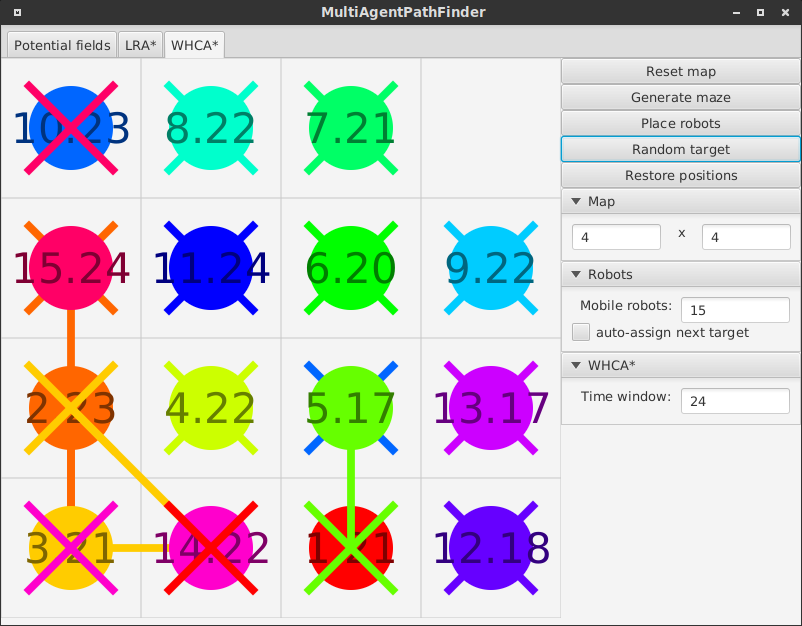
\includegraphics[width=0.8\columnwidth]{img/robopath/puzzle-15}
	\caption{Metoda WHCA*: puzzle 15}
	\label{fig:test-puzzle-15}
\end{figure}

przykład chowania się robotów (przepuszczania się VIPów) - z zaznaczeniem i opisem tras

\section{Dyskusja wyników}
LRA: wyszło całkiem nieźle w przypadku, gdy do celu prowadzi wiele alternatywnych ścieżek i można ominąć wąskie gardło
potwierdzenie oczekiwań (poprawności) - nigdy nie było tak, żeby LRA był lepszy

wolno działa WHCA* przy dużych mapach / oknach czasu / robotach. Dałoby się zoptymalizować (RRA)
autorski WHCA* działa dobrze nawet przy rozwiązywaniu dużych deadlocków, problem z puzzle 15

wada - nie moze się dwóch agentów "cofać". MOże tylko uciekać  z drogi ważniesjzemu